\section{The \instname\ data reduction flow.}
\label{sec:reduction_flow}


The overall data flow of the \instname\ pipeline is displayed in Figure \ref{fig:reduction_cascade}.

 
\begin{figure}[h!]
\centering

\includegraphics[width=0.9\textwidth]{../instrument_tutorial/figures/reduction_cascade.jpg}
\caption{The data reduction cascade of the \instname\ workflow.}
\label{fig:reduction_cascade}
\end{figure}



The reduction cascade is organized in tasks, which represent
well-defined steps in the process. Tasks can be grouped inside
sub-workflows.  Each task runs a recipe; the detailed description of
the algorithms, input, outputs and recipe parameters used in each
recipe are available in the pipeline manual. Here, we present only the
description of most important features.

The \wkfname\  \edps\ workflow is designed to execute the tasks that
deliver the final reduced data cube for each dataset. It can be either
the product of a single exposure, or the combination of multiple
exposures. Only calibrations needed by the selected the scientific
exposures are processed.

It is possible to set \edps\ to perform the data reduction until a
certain step of the reduction chain (e.g. to reduce only standar
stars, or only flat fields).  This is done by specifying the desired
tasks in the field {\bf Select reduction target} of the {\bf Raw Data}
tab.

The reduction steps of the \wkfname\ workflow are listed below. Before
starting the reduction, the parameters of the recipes associated to
each task can be configured by pressing the button

\includegraphics[width=0.8cm]{../common/figures/configure_dataset.jpg}
close to each dataset configuration.
See for more info on the configuration editor \ref{sec:configuration_editor}





The EDPS data reduction workflows process data in batches, called datasets, consisting of related science observations and the necessary calibrations. Therefore, the first steps in executing an EDPS data reduction workflow are to classify the input data and organize it into datasets. ESPRESSO follows the pattern adopted for many instruments designed for RV monitoring: each dataset includes only a single science observation (and all necessary calibrations for its processing) and each dataset is processed by the pipeline recipes separately, generating a product for each raw input file.

Next comes the processing of calibrations. Only those that are needed by the selected scientific exposures are processed.

Finally, the science data are processed and, as explained, a product is generated for each individual dataset, which is equivalent to a product for each individual raw science file. However, ESO provides a set of additional recipes grouped in ESO Tool Kit (ESOTK) that includes a recipe {\tt esotk\_spectrum1d\_combine} designed to combine 1-dimensional spectra (in the ESO internal data product format; the \instname\ pipeline products are already in this format, so there is no need for conversion). The  \wkfname\  workflow uses this recipe to generate a combined spectrum of multiple exposures.
By default, exposures of the same template are selected for combination. To skip combination, deselect the {\bf combine\_science} task from the Reduction Targets field in item 3 (Select the reduction target) of the Raw Data tab.  




The reduction steps of the  \wkfname\  workflow are:

\subsection{Detector properties}

The processing begins with the usual detector-related manipulations
(bias, dark, detector monitoring), marked with the rectangle in 
the top row and performed in a separate subworkflow, named Detector properties (see Figure \ref{fig:espresso_wkf_Detector_01}).



\begin{figure}[h!]
\centering
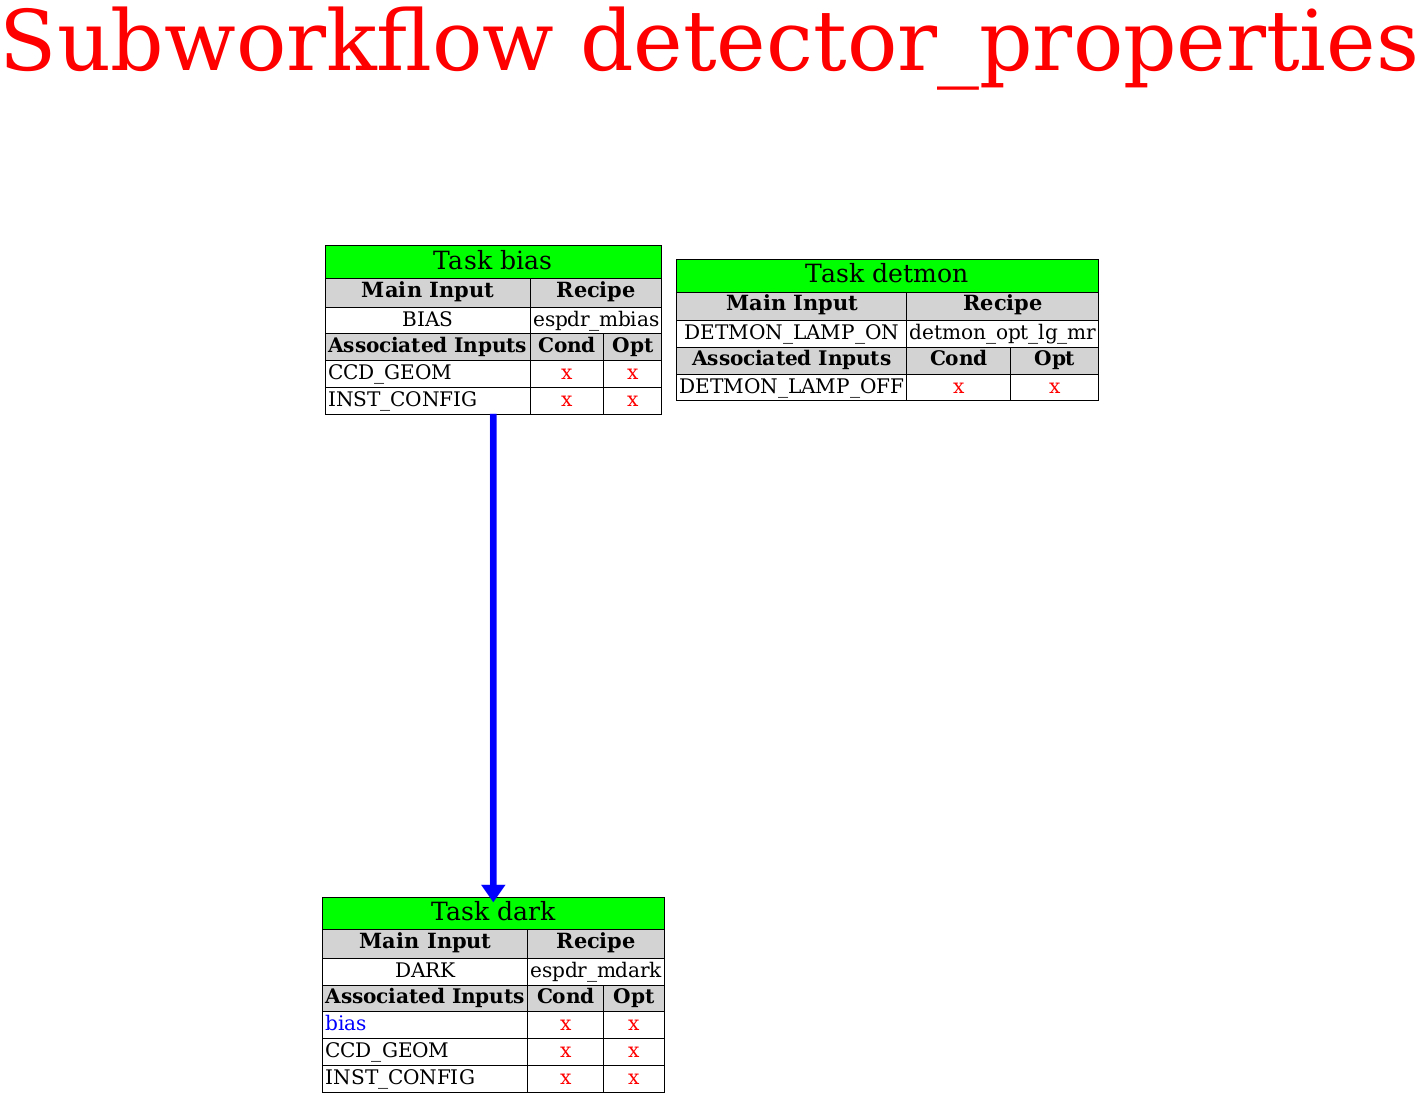
\includegraphics[width=0.7\textwidth]{figures/espresso_wkf_Detector_01.jpg}
\caption{The list of tasks and their dependencies in the detector properties subworkflow.}
\label{fig:espresso_wkf_Detector_01}
\end{figure}



It includes the following tasks {\bf bias} (recipe {\tt espd\_mbias}, for the master bias and bad pixel mask)
{\bf detmon} (recipe {\tt detmon\_opt\_lg\_mr}, for the linearity correction if the detmon package
is installed) and {\bf dark} (recipe {\tt espdr\_dark}, for the master dark and the hot pixel mask).

Graphical reports for the products of tasks {\bf bias} and {\bf dark}
can be inspected. Recipe parameters that control the stacking method
or the sigma clipping can be used if needed, but typically default
parameters provide the best results.

\subsection{Flats and tracing}

This subworkflow is dedicated to generate the flat fielding, the blaze
function, and to trace and identify the various dispersion orders of
the fibre spectra on the detector (Figure
\ref{fig:espresso_wkf_FlatTracing_01}).


\begin{figure}[h!]
\centering
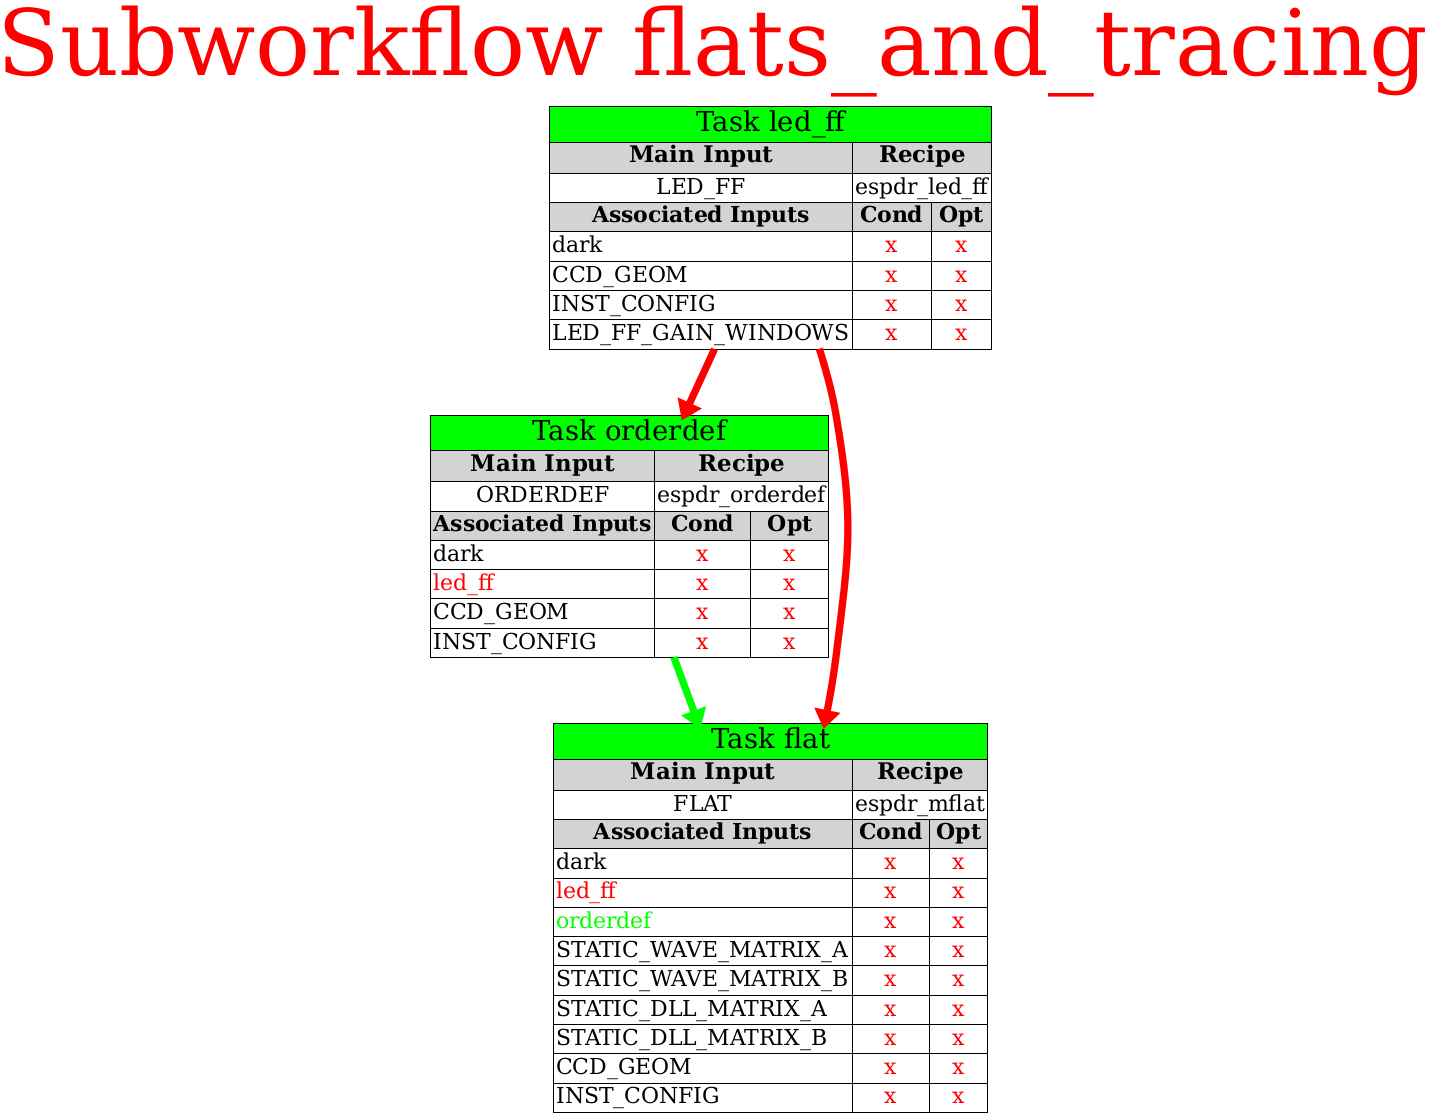
\includegraphics[width=0.7\textwidth]{figures/espresso_wkf_FlatTracing_01.jpg}
\caption{The list of tasks and their dependencies in the flats and tracing subworkflow.}
\label{fig:espresso_wkf_FlatTracing_01}
\end{figure}


It contains the tasks {\bf led\_ff} (recipe {\tt espdr\_led\_ff}), {\bf orderdef} (recipe {\tt espdr\_orderdef}), and task {\bf flat} (recipe {\tt espdr\_mflat}).



The products from these and the previous recipes are used across the
rest of the ESPRESSO workflow, as can be seen from the arrows that
connect them with the following recipes and sub-workflows.

Graphical reports for the products of the tasks {\bf orderdef} and
{\bf flat} can be inspected. Tipicallt, the default recipe parameters
provide already the best results.



\subsection{Wavelength calibration}

This subworkflows executes all the steps and the tasks to compute the
wavelength calibration of \instname\ data (Figure
\ref{fig:espresso_wkf_Wavl_01}).

The wavelenght solution is computed wavelength calibration using
various calibration sources, and illuminating both fibres with them,
on a combination that depends on the observing strategy.

The task {\bf wave\_fp\_fp} runs the recipe {\tt espdr\_wave\_FP} to
process calibrations that have both fibres illuminated by the the
Fabry-Pérot etalon lamp.

The tasks {\bf wave\_fp\_thar} and {\bf wave\_thar\_fp} run the recipe
{\bf espd\_wave\_THAR}, to process calibrations that have one fibre
illuminated by the Fabry-Pérot and the other illuminated by the
Thorium-Argon lamp.

There is also an option of laser frequency comb-based wavelength
calibration via the tasks {\bf wave\_fp\_lfc}, {\bf wave\_lfc\_fp}
(recipe {\tt espdr\_wave\_LFC}). The LFC is a preferable wavelength
calibration method for programs aiming to obtain accurate radial
velocities (RV), because ThAr lamps degrade with time, leading to
larger RV scatter. However, the ThAr provides a first guess for
deriving the LFC solution, which explains the sequence of tasks in the
workflow.


\begin{figure}[h!]
\centering
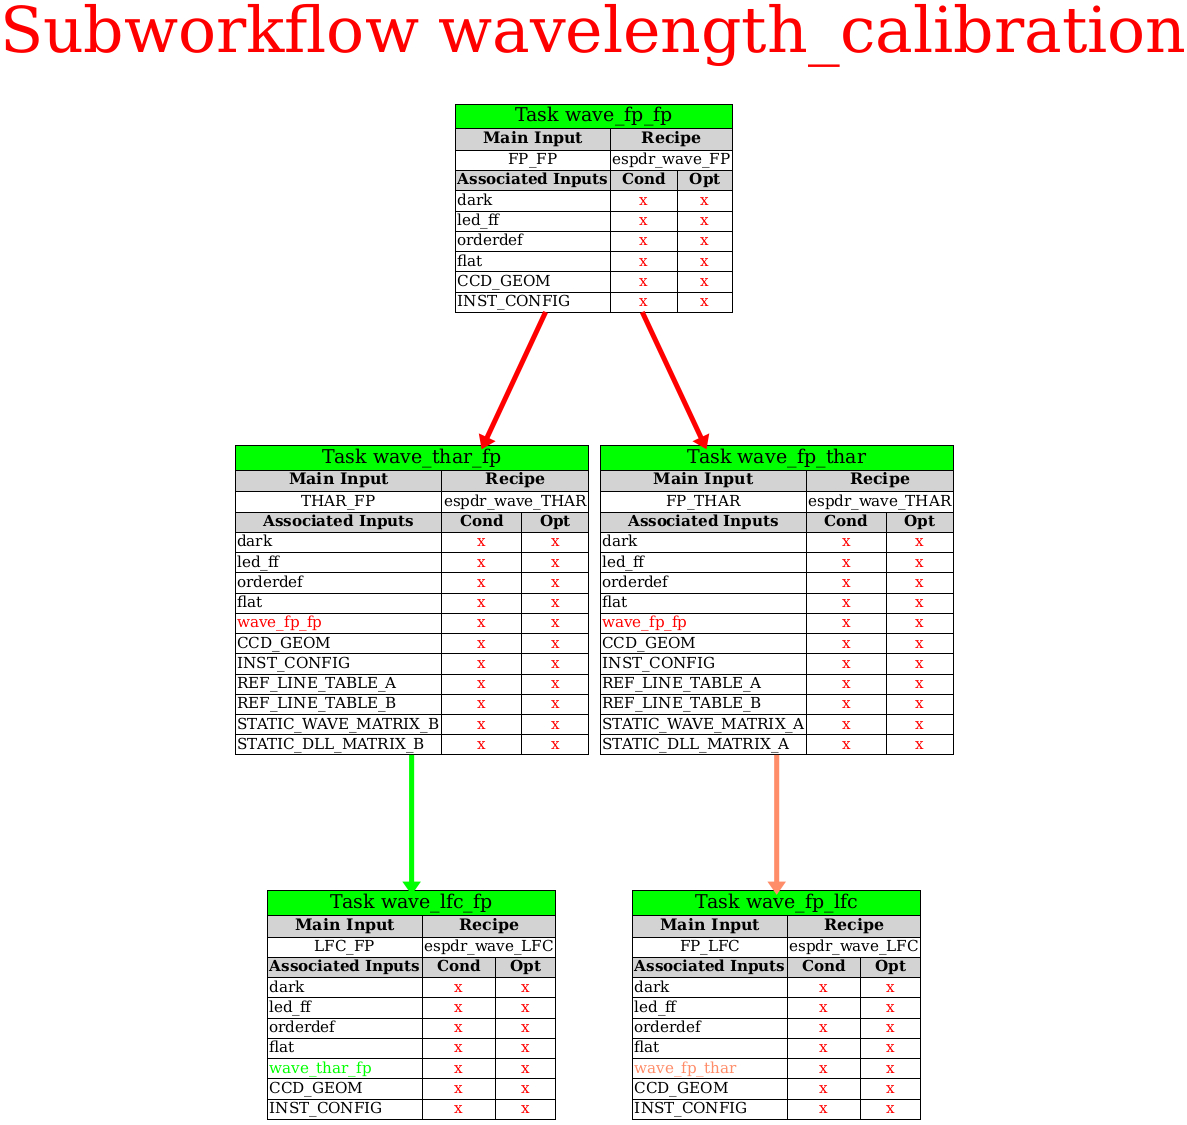
\includegraphics[width=0.7\textwidth]{figures/espresso_wkf_Wavl_01.jpg}
\caption{The list of tasks and their dependencies in the wavelength calibration subworkflow.}
\label{fig:espresso_wkf_Wavl_01}
\end{figure}

Graphical reports for the products of all the tasks can be inspected; typically the recipe default parameters already provide the best results.


\subsection{comtam\_thar, contam\_fb, eff\_ab}
These tasks computes the fibre contamination when illuminated by the
Thorium-Argon and Fabry-Perot lamps (recipe {\tt espdr\_cal\_contam}), and the mutual contamination
between the two fibres (recipe {\tt espdr\_cal\_eff\_ab}). Tipically, default values give the best
results.


The user may change parameters controlling the overscan determination, the inter-order background computa-
tion, and the extraction. The user may change the parameters that control the overscan, the inter-order back-
ground determination, the extraction and the polynomial fit degree used to fit the efficiency

Occasionally, cosmic rays might cause a bad result. In this case, it
is recommended to clean the raw contaminated frames via external tools before processing
them with edps.


\subsection{Flux}

The task {\bf flux} runs the recipe recipe {\bf espdr\_cal\_flux}, and
generates the response curve that converts the flux conversion into to
ergs s$^{-1}$ cm$^{-2}$ \AA$^{-1}$, based on a flux standard
observation; it can also correct for the extinction.

Default recipe parameters generally provide the best results, but the
user may change the parameters that control the overscan, the
inter-order background determination, the extraction and the
polynomial fit degree used to fit the efficiency.


\subsection{Science Reduction}
The subworkflow science reductions processes science data and radial velocity standard using the recipe {\tt espdr\_sci\_red} in the tasks {\bf object} and {\bf rv\_stars}

The two tasks performs the same steps on different types of data, therefore the folloing applies to both of them.


\subsubsection{Sky subtraction}

For very low S/N regime, readout limited or close to it, it is
recommended to use the option smooth for sky subtraction, thus
reducing the readout noise contribution from the step of sky
subtraction. This can be done by setting the recipe parameter {\tt
  sky\_corr\_method} to {\tt smoothed} in the configuration editor.


\subsubsection{Background intra-order contamination}

The recipe parameter {\tt background\_sw} removes the intra-order
diffuse background contamination (it does not have to be
mis-interpreted by sky background, which is regulated by {\tt
  sky\_sub\_method} and active only for OBJECT,SKY observations). It
is evaluated on boxes of size {\tt sci\_bkgr\_grid\_size\_x} $\times$
{\tt sci\_bkgr\_grid\_size\_y} and then interpolated all over the
frame. The diffuse background is proportional to the dispersed light
inside the spectrograph (and thus, to a good approximation, to the
total flux recorded in the detector). If the diffuse back- ground is
not measured correctly (as happens when is negligible), correcting for
it will only add an additional source of noise to the
flux. Fabry-Perot light contributes significantly to the inter-order
background and as such exposures with FP on fiber B have the
inter-order background correction flag by default at ON. In most
cases, stellar light does not contribute significantly to inter-order
background and as such exposures with SKY on fiber B have the
inter-order background correction flag by default at OFF. If any
exposure points to the SKY on fiber B and yet has a very large target
flux in fiber A, the user should change the inter-order correction
flag to ON.

\subsubsection{Radial velocity}
The computation of radial velocity is a key-feature in the
\pipename\ pipeline. One might decide to fine-tune the recipe
parameters to improve the calculation or to run a dedicated esoreflex
workflow and recipe to execute only this step: they are available as
part of the ESPRESSO-DAS pipeline, which is capable of dealing also
with \instname\ data. We refer the user to the ESPRESSO-DAS
documentation for this option.

The recipe parameters that optimize the computation of radial velocity
are: {\tt rv\_range} and {\tt rv\_step}.  The general recommendation is
to start with a large range {\tt rv\_range} and a course grid {\tt
  rv\_step} to locate the minimum. Then a fine-tuning of the range and
grid are necessary to increase the precision of the measurement.
However, M-dwarfs are particularly prone to bad convergence in the CCV
computation if the RV range is large.  It is not recommended to derive
RVs using an RV range larger than 20 km/s for M dwarfs.  When
computing the radial velocity of the same target over a certain period
of time, it is important to use the same template (mask\_table\_id) to
remove systematic effects between measurements at different epochs.

The quality can be checked by inspecting the CCF product (see
\ref{sec:products}) and check whether a clear minimum is visible over
the individual orders.

Figure \ref{fig:ccf} show an example of bad and good CCF computations.



\begin{figure}[h!]
\centering
\includegraphics[width=0.9\textwidth]{figures/ccf.jpg}
\caption{Examples of CCF. The left panel shows a CCF with a well defined minimum over the orders; the right panel shows a CCF with undefined minimum over the orders. In this latter case, the initial guess of the velocity was way off the analized range specified by  {\tt rv\_range}.}
\label{fig:ccf}
\end{figure}



\subsubsection{Cosmic rays cleaning}

The science recipe has two algorithms for cosmic ray cleaning. They
user can decide to use none, one or both by setting the corresponding
recipe parameter in the configuration editor.  The parameters are:
\begin{itemize}

\item {\tt ksigma\_cosmic}. ksigma for removing cosmics on fiber A or
  SKY; Set it to -1 to deactivate it. Default: 3.5. The algorithm
  operates on the extracted spectrum and flags pixels that deviate
  more than a certain factor.
  
\item {\tt cosmic\_detection\_sw}. Use the LA Cosmic detection (van
  Dokkum 2001, PASP 113, 1420). Set it to 0 to disable, 1 to enable.
  {\tt cosmic\_detection\_sw} to 1 or 0, respectively. Pixels that are flagged
  are ignored during the extraction of the one-dimensional
  spectrum. The tab “LACOSMIC” in the interactive window allows the
  user to specify the recipe parameters that control the algorithm. By
  default, the workflow switches on/off the algorithm and loads the
  optimal recipe parameters for a given observing mode. We refer the
  user to the pipeline manual for more information on the recipe
  parameters. The user might want to inspect the products with
  category CRH\_MAP and CCD\_CORR\_SCIENCE to assess the quality of
  the flagging process. These products are available by pressing the
  magnifying glass of the corresponding job.
 
\end{itemize}

The general recommendation is to switch on both algorithms, but pay
attention whether very intense targets or very intense exposures of
fibre B (in particular with high binning modes), do generate too many
false positive detections. In this case, it is recommended either to
switch the LA Cosmic algorithm off, or to increase the {\tt f\_lim}
{\tt sigma\_lim} thresholds, regulated by the corresponding recipe paramters.

If a cosmic ray is only partially detected, one might dilate the
cosmic-ray mask by setting recipe parameters {\tt post-filter-x} and
{\tt post-filter-y} parameters to 1 or 2 (higher values are not
recommended).


The user has the option to provide a mask with cosmic rays detection (category CRH\_MAP). If provided, it will
switch off the execution of the LA Cosmic algorithm. In order to be used by the workflow and the recipes, the
user-provided mask has to:
\begin{itemize}
\item be present amon the inputs.
\item have the category {\tt CRH\_MAP} (header keyword HIERARCH ESO PRO CATG).
\item have the same format of {\tt CRH\_MAP} produced by switching on the LA Cosmic algorithm. The convention is: pixels
with value of 1 are cosmic rays, other pixels have value 0 (integers).
\item have the header keyword ARCFILE of the same value of the science frame it is supposed to be associated
  to.
  \end{itemize}
It is therefore recommended to first run the reduction with the LA Cosmic algorithm turned on, with the option
{\tt extra\_products\_sw}, and then edit the CRH\_MAP produced by the workflow according to the needs. It
is also possible to run a third-party cosmic ray detection algorithm on CCD\_CORR\_SCIENCE and record the
flagged pixel into CRH\_MAP.
Note that the inclusion of an user-provided CRH\_MAP replaces the LA Cosmic algorithm in the science recipe,
but the “k-sigma clipping” algorithm can still be executed.


\subsubsection{Products}
\label{sec:products}

In general, the products of the science reduction subworkflow follow two formats:

\begin{itemize}
\item One dimensional spectra or S1D. They are FITS tables that
  consist of a header with no data and a regular FITS table stored in
  the first extension (and can be inspected with any tool that reads
  FITS tables, such as topcat or fv). The combine the information of
  several orders. The column names in the table vary depending on the
  product type. Information about some columns that can be found in
  the S1D tables (e.g., in the S1D\_FINAL\_A files) is given in Table 2,
  and a plot of the S1D spectrum, generated with EDPS, is shown in
  Figure \ref{fig:s1d_example_plot_01} and in the bottom panel of
  Figure \ref{fig:s2d_example_plot_01}.
  
\item Two dimensional spectra, or S2D. They show in each row the
  spectrum of each order. It has multiple extensions, the first
  extension contain the spectra, other extensions contain the
  wavelength information (vacuum and air in separate extensions),
  errors, and quality flags. The wavelength runs horizontally across
  the order, increasing from left to right, but it is stored in one of
  the extensions, so normally the files are displayed in pixels. The
  bluest orders are located at the bottom, and they are shorter than
  the reddest orders which are located on the top – this is due to the
  specifics of the ESPRESSO optical design. These files are
  2-dimensional images, and they can be inspected with any image
  display tool such as fv or ds9. An example of S2D quality plot is
  shown in Figure \ref{fig:s2d_example_plot_01} (top panel).

\item Other products, such as
  \begin{itemize}
    \item CCF\_A. Cross correlation function for fibre A with the
      object in S2D format. It contains the CCF for each order, with
      the corresponding errors and the data quality (in separate FITS
      extensions).
    \item CCF\_RESIDUALS\_A Residuals from CCF computation of the RV
      for the spectrum – a FITS table with RVs, their errors and the
      residuals from the mean RV for each individual order of the
      spectrum.
   \item DRIFT\_MATRIX\_B. Drift matrix in S2D format with a single
     extension, storing the relative shift of the wavelength
     calibration solution position of the spectrum in fibre A (with
     the science target) relative to fibre B (with the calibration
     source) between the time of (night) observation and the time when
     the calibration was acquired (during the day).	
   \item S2D\_BLAZE\_A/B Blaze functions on order-by-order basis for
     fibre A/B.
\end{itemize}
  \end{itemize}

A full list of products and their description is given in the pipeline
manual. It is worth showing here the columns present in the extracted
spectra (Table \ref{tab:s1d_product}).

\begin{table}[htbp]
\centering
\caption{An example of the ESPRESSO S1D product spectra.}
\label{tab:s1d_product}
\small
\begin{tabular}{|l|l|p{9cm}|}
\hline
\textbf{Column name} & \textbf{Units} & \textbf{Description} \\
\hline
WAVE & [\AA] &
Wavelength vector, in vacuum reference system. \\
\hline

FLUX & [erg cm$^{-2}$ s$^{-1}$ \AA$^{-1}$] or [e$^{-}$] &
Flux of the final extracted spectrum in Fibre A, fully reduced till the end of the data reduction cascade. It is flux calibrated (if flux calibration was performed) and sky subtracted (if sky subtraction was performed). \\
\hline

ERR & [erg cm$^{-2}$ s$^{-1}$ \AA$^{-1}$] or [e$^{-}$] &
Error associated to FLUX. \\
\hline

QUAL & &
Quality flag associated to FLUX. \\
\hline

SNR & &
Signal to noise ratio, obtained from FLUX/ERR. \\
\hline

WAVE\_AIR & [\AA] &
Wavelength vector, in the air reference system. \\
\hline

FLUX\_EL & [e$^{-}$] &
Extracted flux from fibre A, not sky subtracted nor flux calibrated. \\
\hline

ERR\_EL & [e$^{-}$] &
Error associated to FLUX\_EL. \\
\hline

QUAL\_EL & &
Quality flag associated to FLUX\_EL. \\
\hline

FLUX\_CAL & [erg cm$^{-2}$ s$^{-1}$ \AA$^{-1}$] &
Extracted flux from fibre A, flux calibrated but not sky subtracted. \\
\hline

ERR\_CAL & [erg cm$^{-2}$ s$^{-1}$ \AA$^{-1}$] &
Error associated to FLUX\_CAL. \\
\hline

QUAL\_CAL & &
Quality flag associated to FLUX\_CAL. \\
\hline

FLUX\_CAL\_SKYSUB & [erg cm$^{-2}$ s$^{-1}$ \AA$^{-1}$] &
Extracted flux from fibre A, flux calibrated and sky subtracted. \\
\hline

ERR\_CAL\_SKYSUB & [erg cm$^{-2}$ s$^{-1}$ \AA$^{-1}$] &
Error associated to FLUX\_CAL\_SKYSUB. \\
\hline

QUAL\_CAL\_SKYSUB & &
Quality flag associated to FLUX\_CAL\_SKYSUB. \\
\hline

FLUX\_EL\_SKYSUB & [e$^{-}$] &
Extracted flux from fibre A, sky subtracted but not flux calibrated. \\
\hline

ERR\_EL\_SKYSUB & [e$^{-}$] &
Error associated to FLUX\_EL\_SKYSUB. \\
\hline

QUAL\_EL\_SKYSUB & &
Quality flag associated to FLUX\_EL\_SKYSUB. \\
\hline

\end{tabular}
\end{table}




\begin{figure}[h!]
\centering
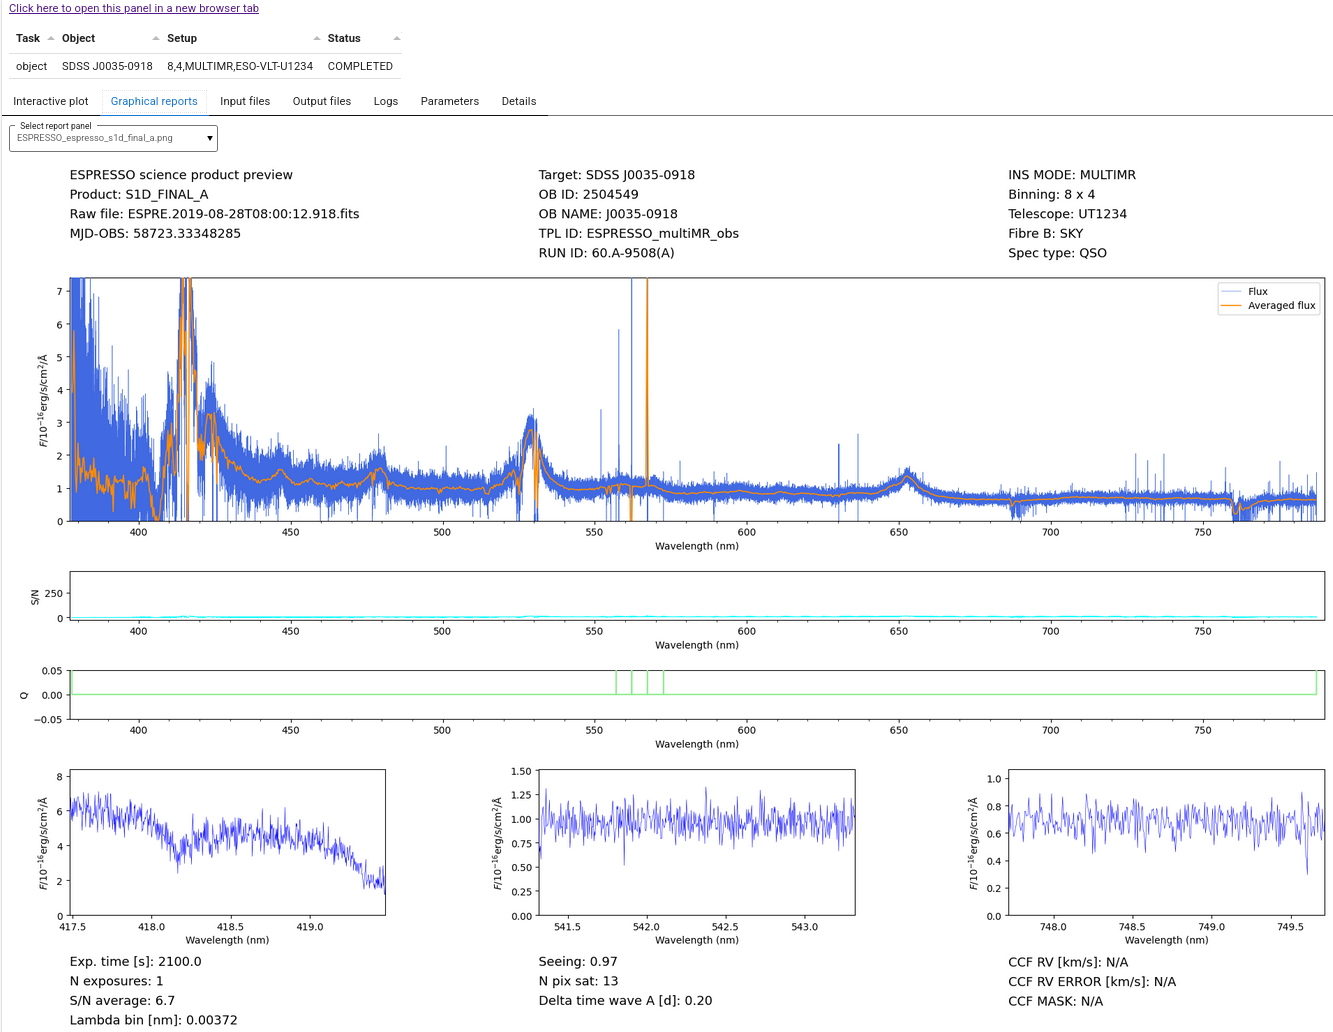
\includegraphics[width=0.7\textwidth]{figures/s1d_example_plot_01.jpg}
\caption{The quality plot (graphic report) associated to the tasks {\bf object} and {\bf rv\_stars}, showing the extracted spectrum (S1D\_FINAL\_A) and zooms on selected regions. A smoothed version of the spectrum is also shown.}
\label{fig:s1d_example_plot_01}
\end{figure}

\begin{figure}[h!]
\centering
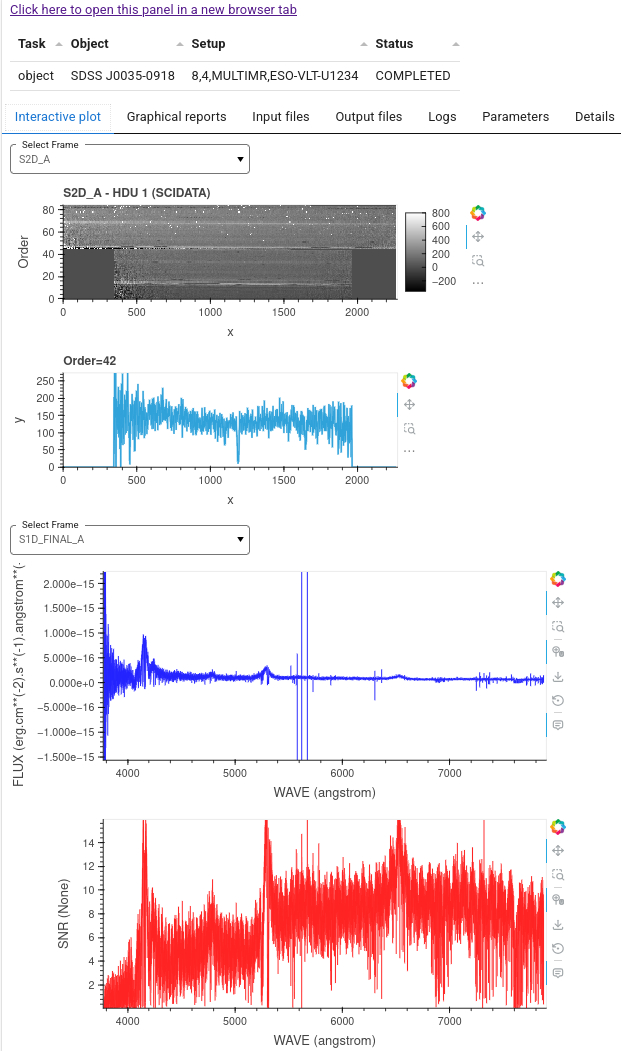
\includegraphics[width=0.7\textwidth]{figures/s2d_example_plot_01.jpg}
\caption{The quality plot (interactive plot) associated to the tasks {\bf object} and {\bf rv\_stars}. Various products can be selected for inspection, in the exaple shown in this figure, the S2D\_A and S1D\_FINAL\_A are shown in the upper and bottom panels, respectively.}
\label{fig:s2d_example_plot_01}
\end{figure}

\subsection{combine science}

This tasks combines the extracted science spectra observed within the
same template using the recipe {\tt esotk\_spectrum1D\_combine}. For studies that implies the study of spectral variation less than 1
hours (the typical OB lenght), it is recommended not to execute it.
